\chapter{Visualizing Neural Networks}


\section{Saliency Map}
\paragraph*{$ \bigstar $ Show and interpret the obtained results.}
After visualizing many saliency maps, most of them were perfectly normal but some were pretty inconsistent. In the following, we will describe each case.

% J'interprète souvent comme "le modèle regarde" alors que la saillancy map est que pour la class prédite et pas pour la ground truth faudrait visu les deux mais du coup pour limiter le nombre de figure mettre moins d'example ? 

\Cref{fig:good_saliency_map} show some consistent saliency maps. When the model make a good prediction, we can see high value on the labelled object. It's the case on all image here exept for the fourth one where the model predicted "greenhouse" instead of "lakeside". In fact, with the fourth image, the model did not focused on the lake frontiers to make this wrong prediction. It has mostly looked on the dark ground and the high brithness part of the image leading to the greenhouse class prediction.
\begin{figure}[H]
    \centering
    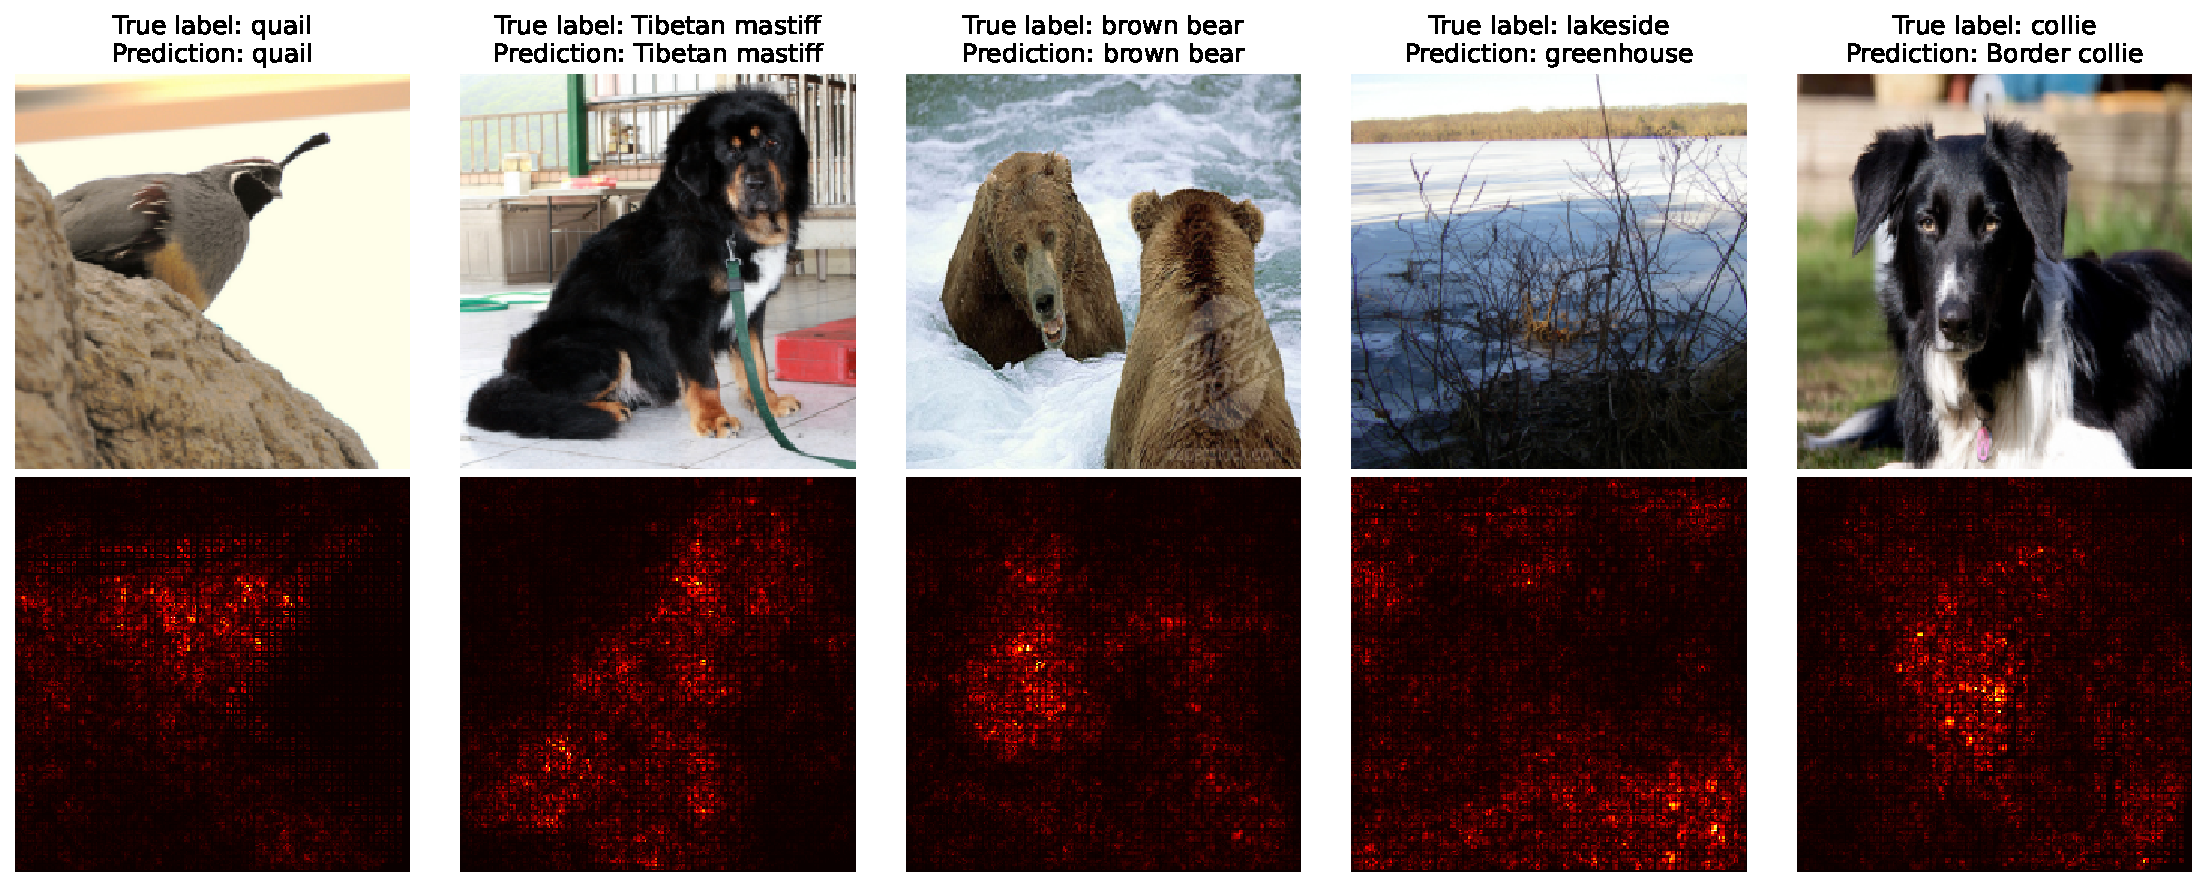
\includegraphics[width=.95\textwidth]{figs/2b/good_saliency_map.pdf}
    \caption{Consistent saliency maps of the predicted class}
    \label{fig:good_saliency_map}
\end{figure}


\Cref{fig:bad_saliency_map} show some saliency maps that we found inconscistent. Both the first and the fourth one are image where the model prediction is correct but the saliency map is not informative at all, kind of blury. For the second and the last image, we can see that the model is looking at the right place but still predict the wrong class.

\begin{figure}[H]
    \centering
    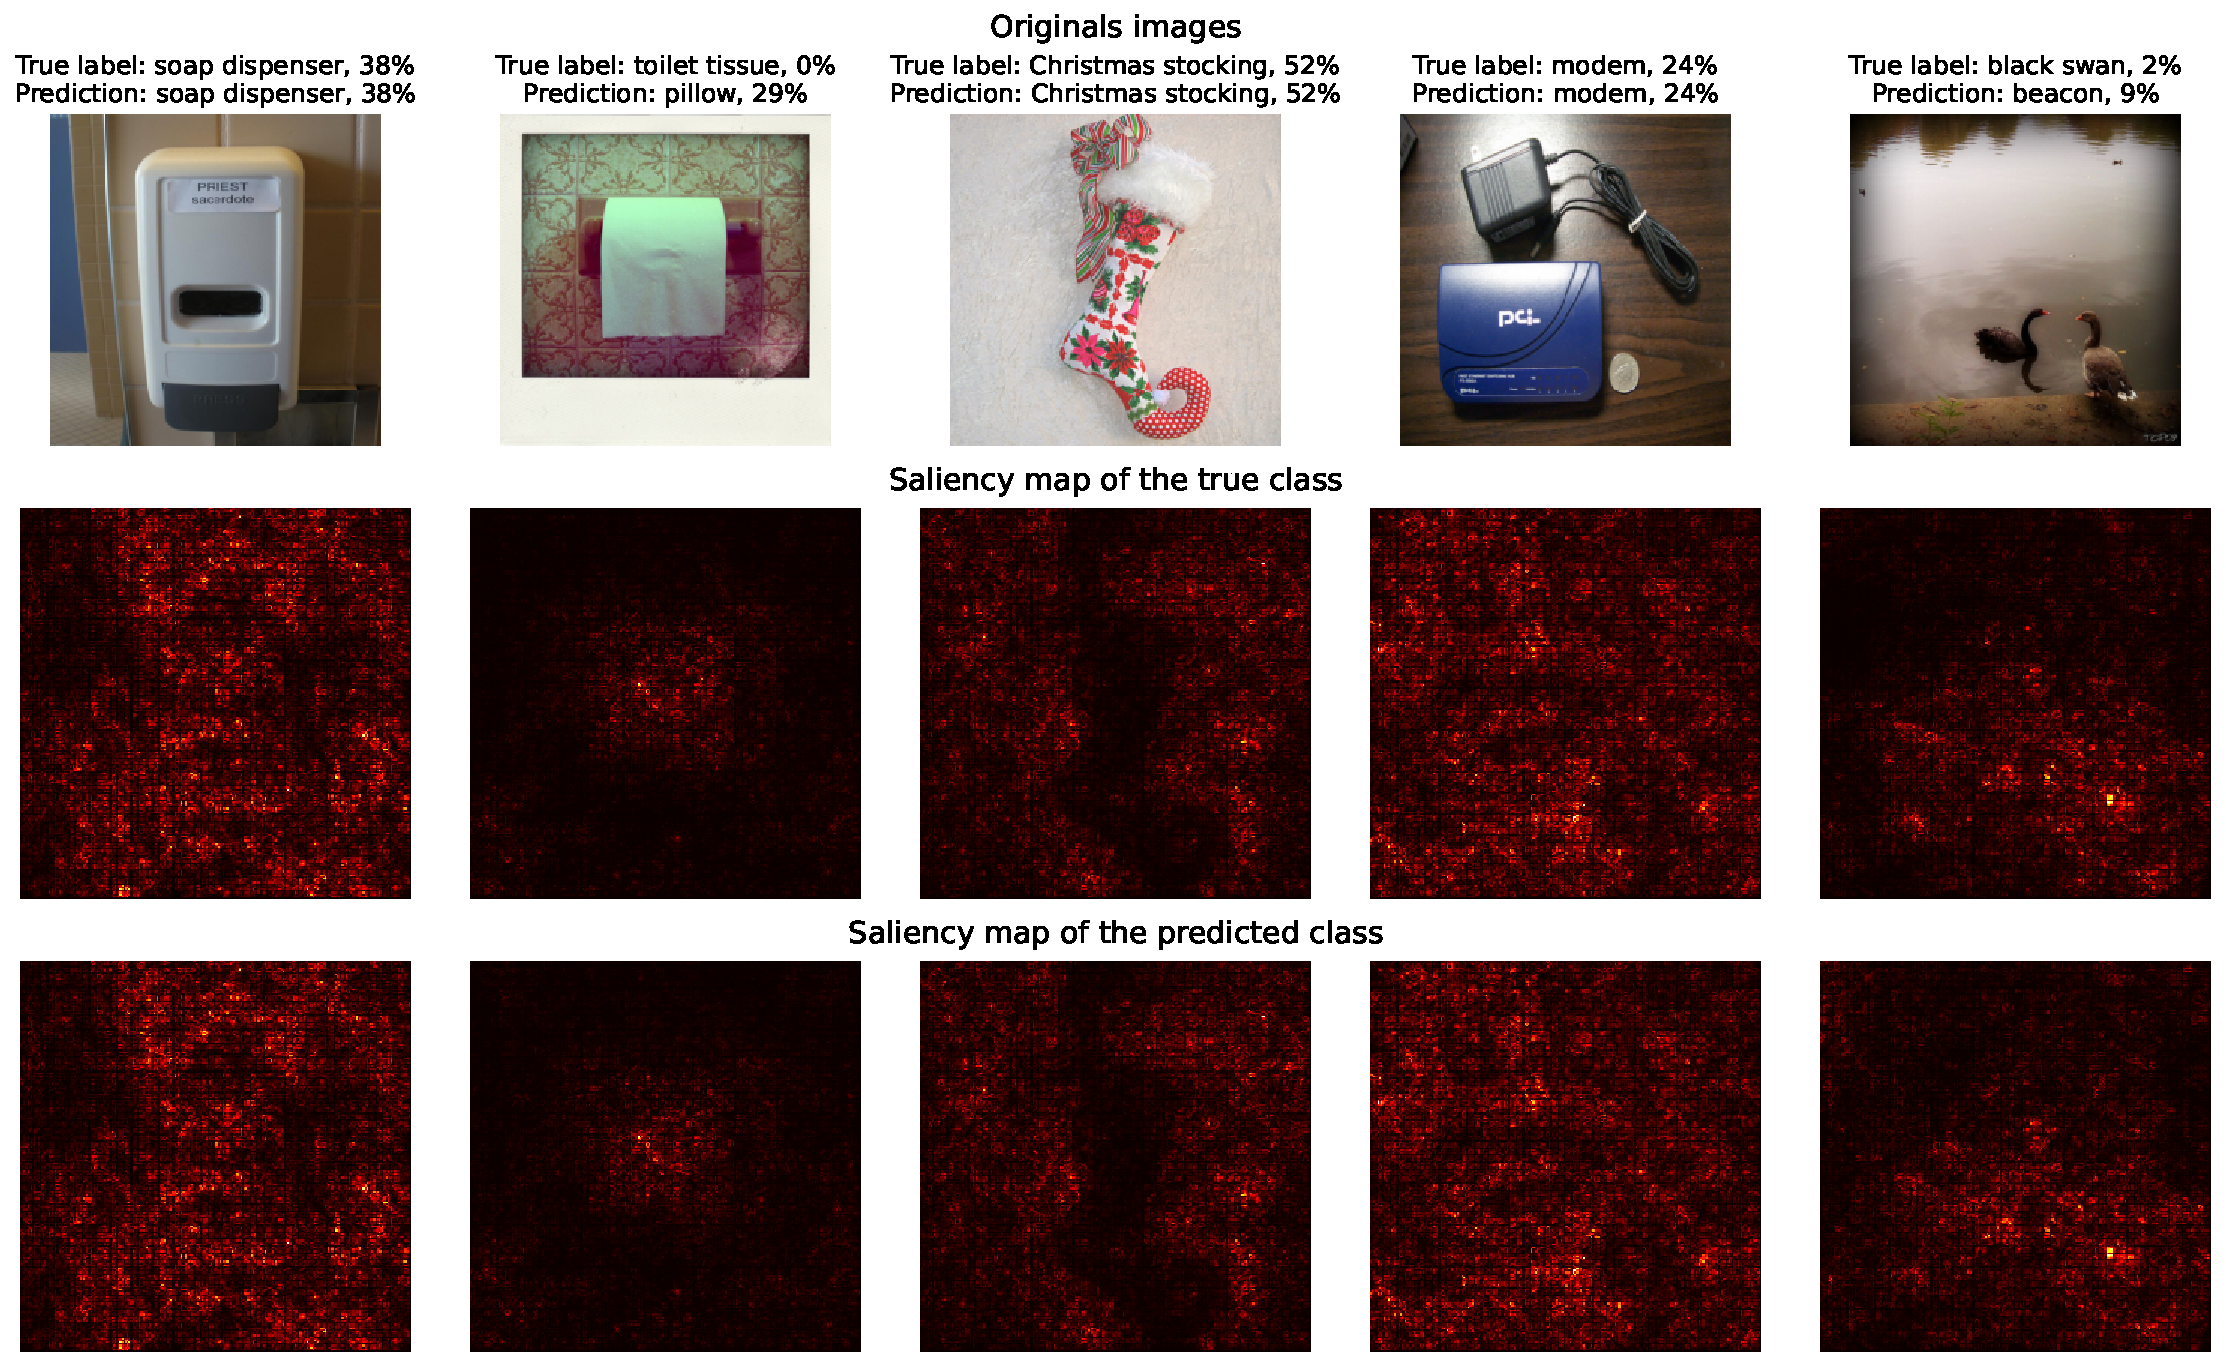
\includegraphics[width=.95\textwidth]{figs/2b/bad_saliency_map.pdf}
    \caption{Inconsistent saliency maps of the predicted class}
    \label{fig:bad_saliency_map}
\end{figure}


\paragraph*{Discuss the limits of this technique of visualization the impact of different pixels.}
\paragraph*{Can this technique be used for a different purpose than interpreting the network ?}
\paragraph*{\textbf{Bonus:} Test with a diffrentent network, for example VGG16, and comment.}



\section{Adversarial Example}
\paragraph*{$ \bigstar $ Show and interpret the obtained results.}
\paragraph*{In practice, what consequences can this method have when using convolutional neural networks?}
\paragraph*{\textbf{Bonus:} Discuss the limits of this naive way to construct adversarial images. Can you propose some alternative or modified ways? (You can base these on recent research)}


\section{Class Visualization}
\paragraph*{$ \bigstar $ Show and interpret the obtained results.}
\paragraph*{Try to vary the number of iterations and the learning rate as well as the regularization weight.}
\paragraph*{Try to use an image from ImageNet as the source image instead of a random image (parameter init\_img). You can use the real class as the target class. Comment on the interest of doing this.}
\paragraph*{\textbf{Bonus:} Test with another network, VGG16, for example, and comment on the results.}